%% ============================================================================================================
%% Results
%% ============================================================================================================
\section{Results}
\label{sec:results}

% Experiment 1. QRF
% ————————————————————————————————————————————————————————————————————————————
\subsection{Experiment 1. Random Forest}
\label{experiment:random-forest}

\begin{figure}[htbp] % Floating specifier: h-here, t-top, b-bottom, p-page of floats
    \centering % Center the entire figure block

    % --- ROW 1 ---
    \begin{subfigure}[b]{0.32\textwidth} % Adjust width as needed (e.g., 0.3\textwidth)
        \centering
        
\includegraphics[width=\linewidth]{bin/shaps/rf/shap_top10_0.pdf} % Replace with your PDF file
        % \caption{Caption for Plot 1}
        \label{fig:plot1}
    \end{subfigure}%
    \hfill % Horizontal fill for spacing between subfigures
    \begin{subfigure}[b]{0.32\textwidth}
        \centering
        
\includegraphics[width=\linewidth]{bin/shaps/rf/shap_top10_1.pdf} % Replace with your PDF file
        \label{fig:plot2}
    \end{subfigure}%
    \hfill
    \begin{subfigure}[b]{0.32\textwidth}
        \centering
        
\includegraphics[width=\linewidth]{bin/shaps/rf/shap_top10_2.pdf} % Replace with your PDF file
        \label{fig:plot3}
    \end{subfigure}

    \vspace{0.2cm} % Optional: Add some vertical space between rows

    % --- ROW 2 ---
    \begin{subfigure}[b]{0.32\textwidth}
        \centering
        
\includegraphics[width=\linewidth]{bin/shaps/rf/shap_top10_3.pdf} % Replace with your PDF file
        \label{fig:plot4}
    \end{subfigure}%
    \hfill
    \begin{subfigure}[b]{0.32\textwidth}
        \centering
        
\includegraphics[width=\linewidth]{bin/shaps/rf/shap_top10_4.pdf} % Replace with your PDF file
        \label{fig:plot5}
    \end{subfigure}%
    \hfill
    \begin{subfigure}[b]{0.32\textwidth}
        \centering
        
\includegraphics[width=\linewidth]{bin/shaps/rf/shap_top10_5.pdf} % Replace with your PDF file
        \label{fig:plot6}
    \end{subfigure}

    \vspace{0.2cm} % Optional: Add some vertical space between rows

    % --- ROW 3 ---
    \begin{subfigure}[b]{0.32\textwidth}
        \centering
        
\includegraphics[width=\linewidth]{bin/shaps/rf/shap_top10_6.pdf} % Replace with your PDF file
        \label{fig:plot7}
    \end{subfigure}%
    \hfill
    \begin{subfigure}[b]{0.32\textwidth}
        \centering
        
\includegraphics[width=\linewidth]{bin/shaps/rf/shap_top10_7.pdf} % Replace with your PDF file
        % \caption{Caption for Plot 8}
        \label{fig:plot8}
    \end{subfigure}%
    \hfill
    \begin{subfigure}[b]{0.32\textwidth}
        \centering
        
\includegraphics[width=\linewidth]{bin/shaps/rf/shap_top10_8.pdf} % Replace with your PDF file
        % \caption{Caption for Plot 9}
        \label{fig:plot9}
    \end{subfigure}

    % \caption{This is the main caption for the entire 3x3 grid of plots. It describes the overall figure composed of subplots (a) through (i).}
    \caption{SHAP values for Random forest}
    \label{fig:shap_rf} % Label for cross-referencing the entire figure
\end{figure}

Figure~\ref{fig:shap_rf} shows the SHAP values for the Random Forest model across all nine clusters. Remarkably, soil moisture level (lvl\_sm) and slope gradient (slp\_dg\_sav) consistently rank highest in importance, while precipitation variability (pst\_pc\_sse) occupies a middle position. This uniform pattern suggests that the model relies mainly on common hydrological drivers rather than on cluster-specific attributes. Such behavior may indicate either insufficient differentiation of clusters by static features or the overwhelming influence of a few key variables in the training data.

% Experiment 2. GBRT
% ————————————————————————————————————————————————————————————————————————————
\subsection{Experiment 2. Gradient boosting}
\label{experiment:GBRT}


\begin{figure}[htbp] % Floating specifier: h-here, t-top, b-bottom, p-page of floats
    \centering % Center the entire figure block

    % --- ROW 1 ---
    \begin{subfigure}[b]{0.32\textwidth} % Adjust width as needed (e.g., 0.3\textwidth)
        \centering
        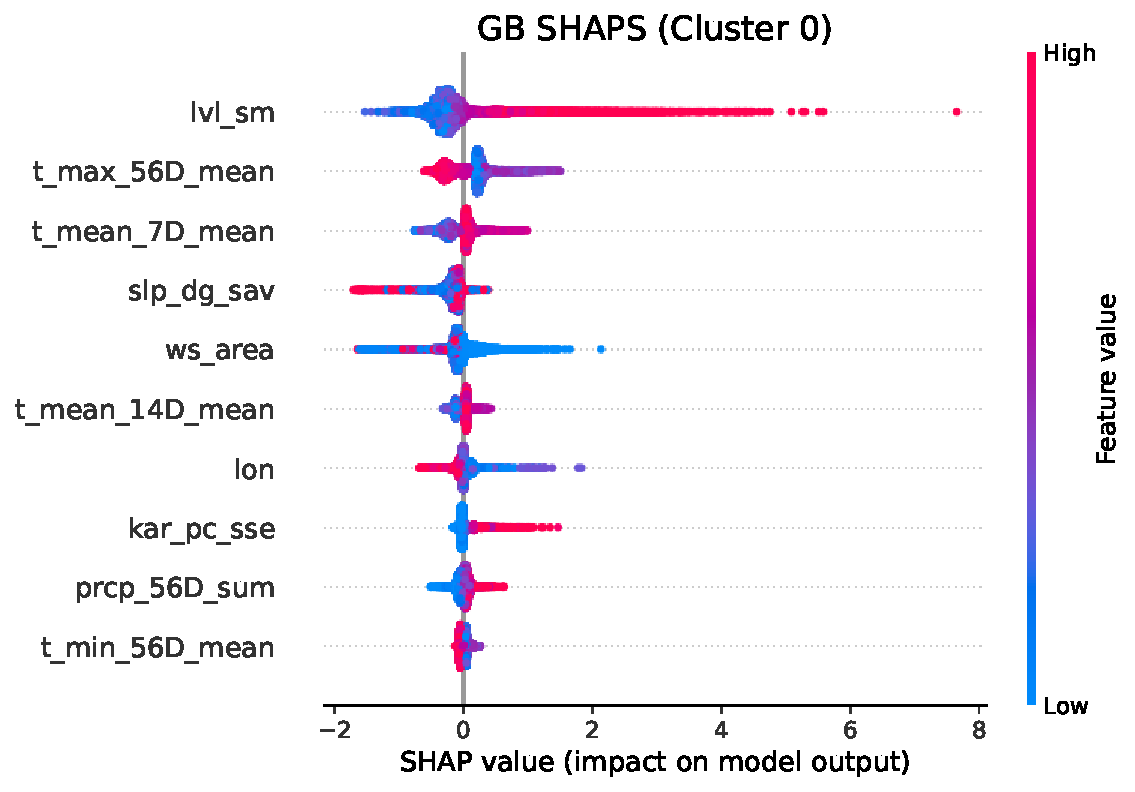
\includegraphics[width=\linewidth]{bin/shaps/gb/shap_top10_0.pdf} % Replace with your PDF file
        % \caption{Caption for Plot 1}

    \end{subfigure}%
    \hfill % Horizontal fill for spacing between subfigures
    \begin{subfigure}[b]{0.32\textwidth}
        \centering
        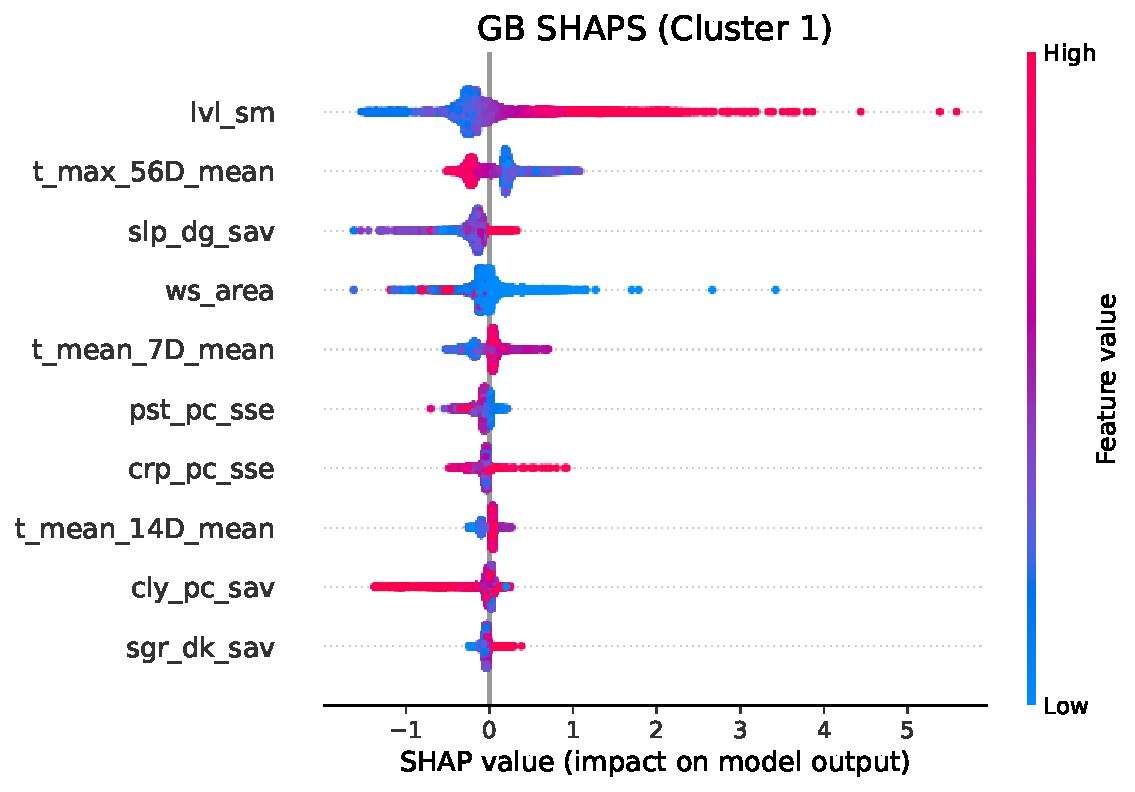
\includegraphics[width=\linewidth]{bin/shaps/gb/shap_top10_1.pdf} % Replace with your PDF file
    \end{subfigure}%
    \hfill
    \begin{subfigure}[b]{0.32\textwidth}
        \centering
        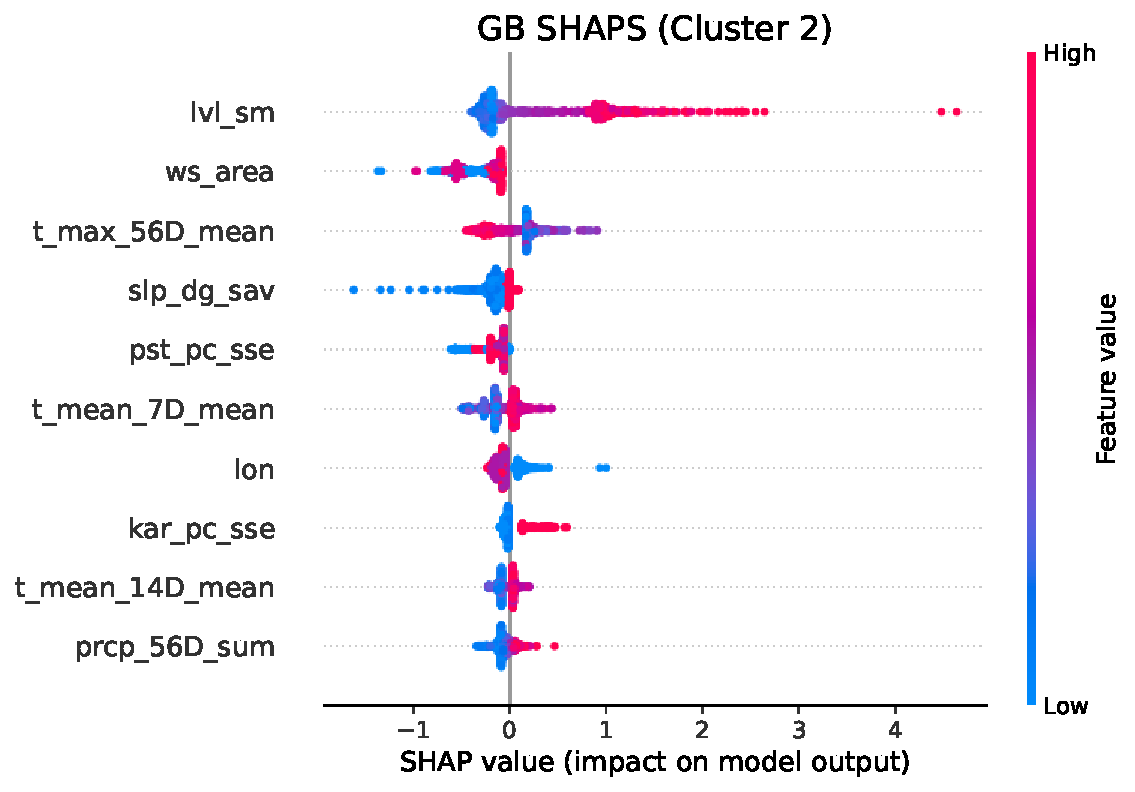
\includegraphics[width=\linewidth]{bin/shaps/gb/shap_top10_2.pdf} % Replace with your PDF file
    \end{subfigure}

    \vspace{0.2cm} % Optional: Add some vertical space between rows

    % --- ROW 2 ---
    \begin{subfigure}[b]{0.32\textwidth}
        \centering
        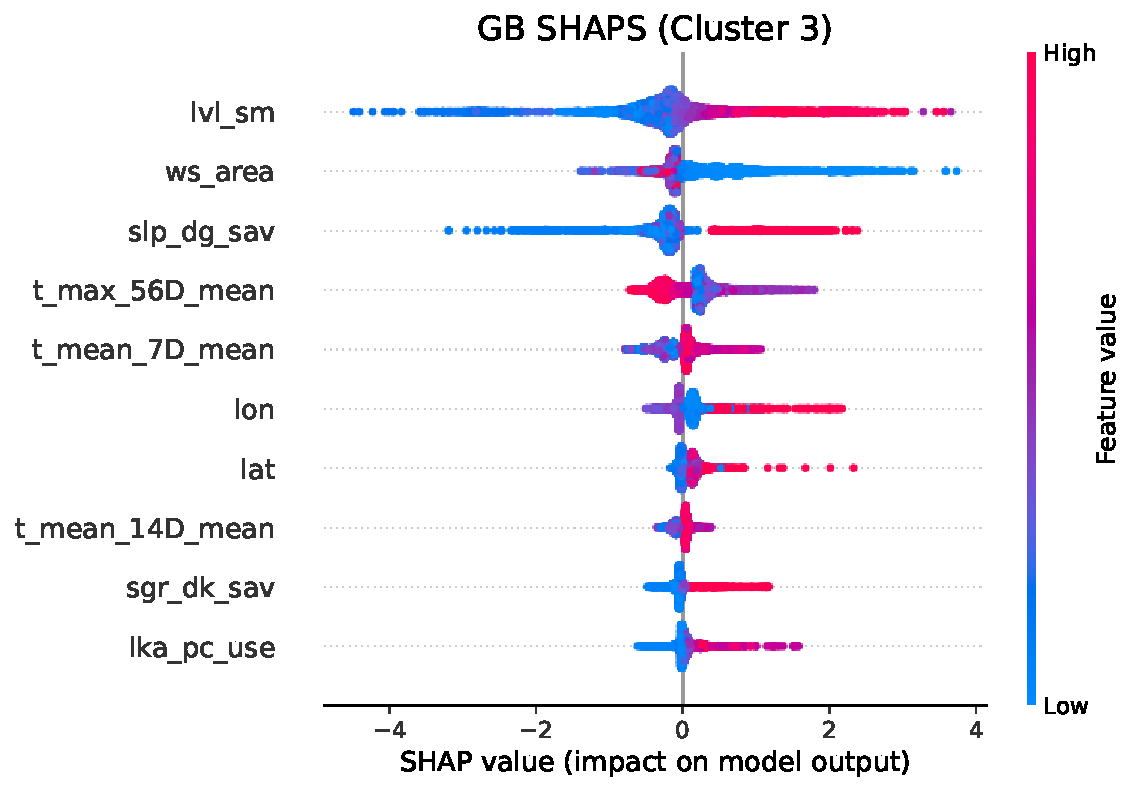
\includegraphics[width=\linewidth]{bin/shaps/gb/shap_top10_3.pdf} % Replace with your PDF file
    \end{subfigure}%
    \hfill
    \begin{subfigure}[b]{0.32\textwidth}
        \centering
        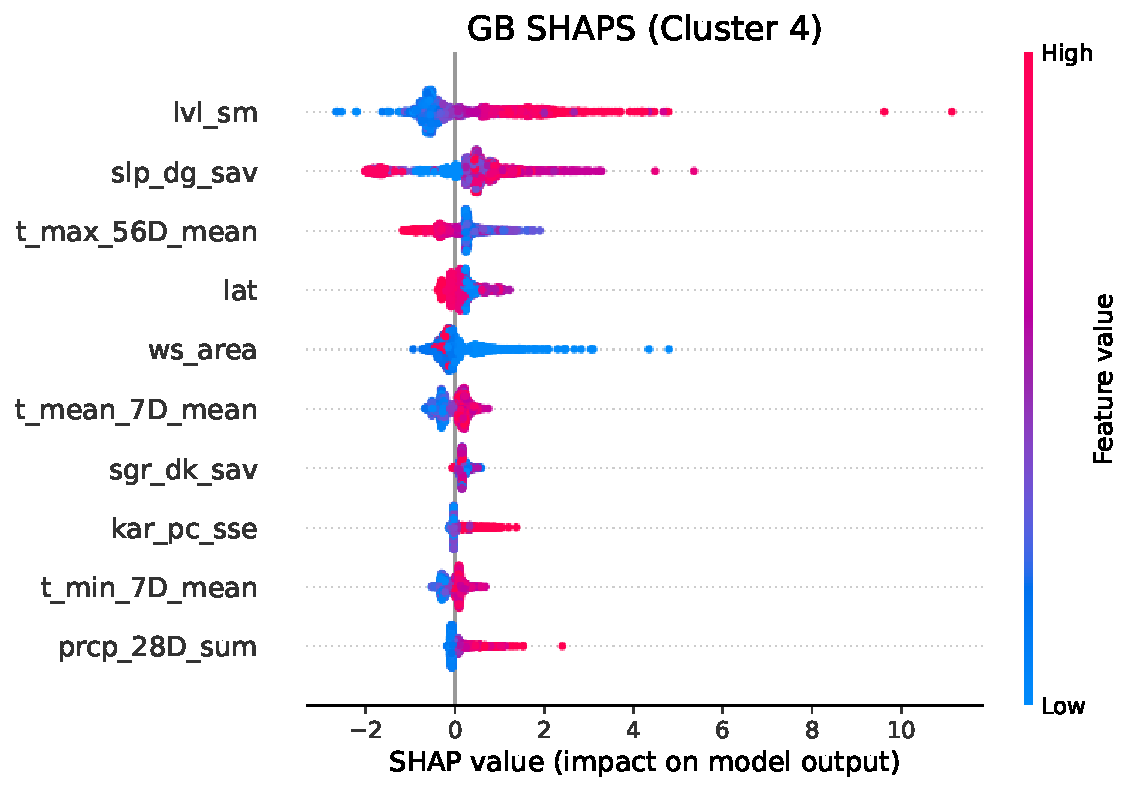
\includegraphics[width=\linewidth]{bin/shaps/gb/shap_top10_4.pdf} % Replace with your PDF file
    \end{subfigure}%
    \hfill
    \begin{subfigure}[b]{0.32\textwidth}
        \centering
        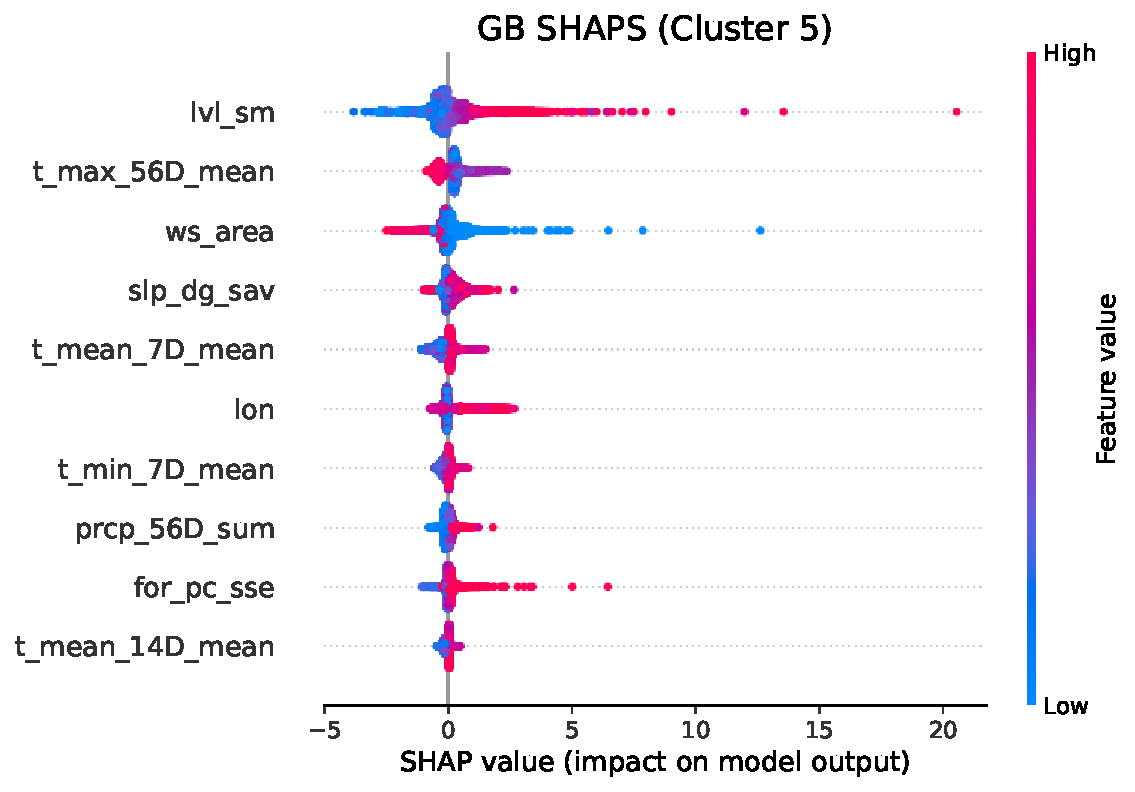
\includegraphics[width=\linewidth]{bin/shaps/gb/shap_top10_5.pdf} % Replace with your PDF file
    \end{subfigure}

    \vspace{0.2cm} % Optional: Add some vertical space between rows

    % --- ROW 3 ---
    \begin{subfigure}[b]{0.32\textwidth}
        \centering
        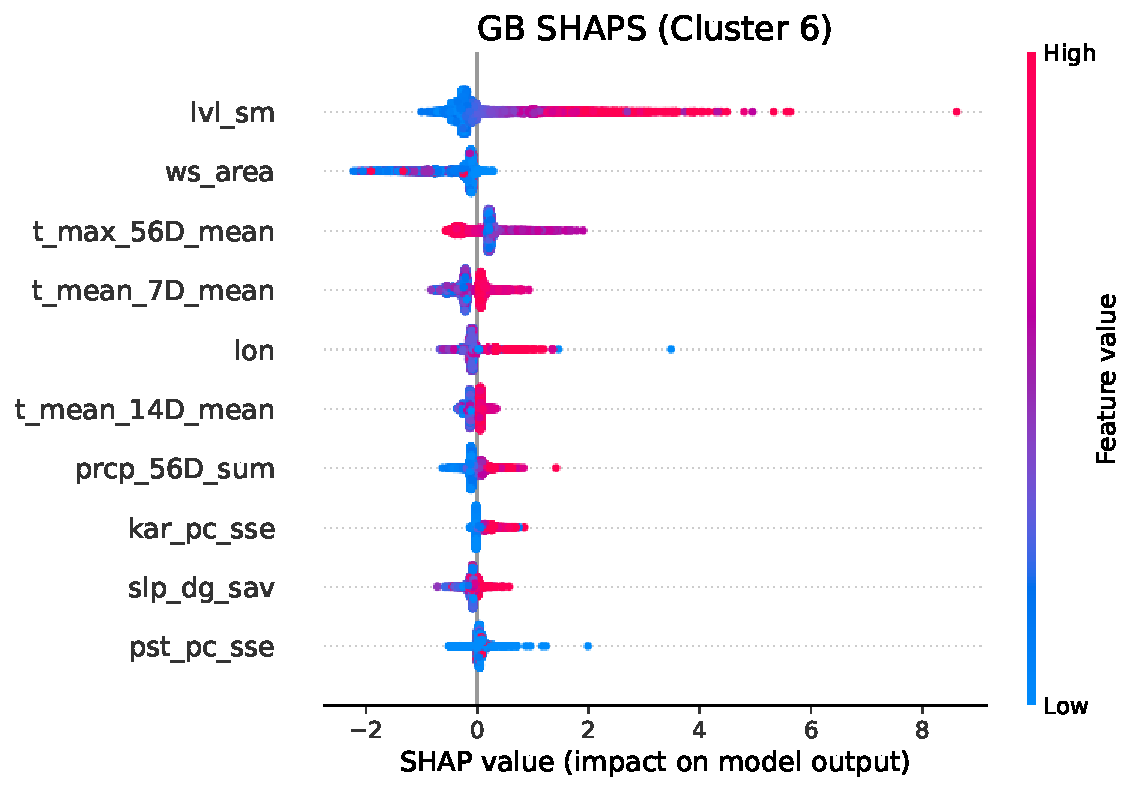
\includegraphics[width=\linewidth]{bin/shaps/gb/shap_top10_6.pdf} % Replace with your PDF file
    \end{subfigure}%
    \hfill
    \begin{subfigure}[b]{0.32\textwidth}
        \centering
        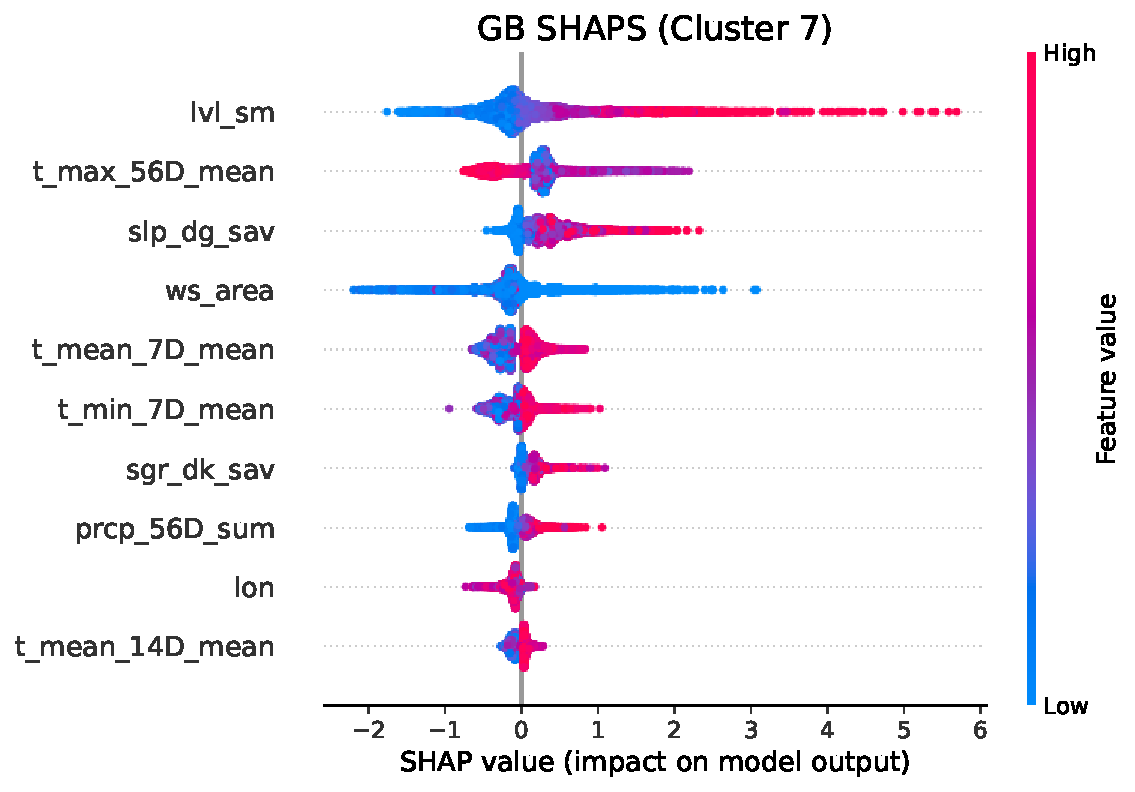
\includegraphics[width=\linewidth]{bin/shaps/gb/shap_top10_7.pdf} % Replace with your PDF file
        % \caption{Caption for Plot 8}
    \end{subfigure}%
    \hfill
    \begin{subfigure}[b]{0.32\textwidth}
        \centering
        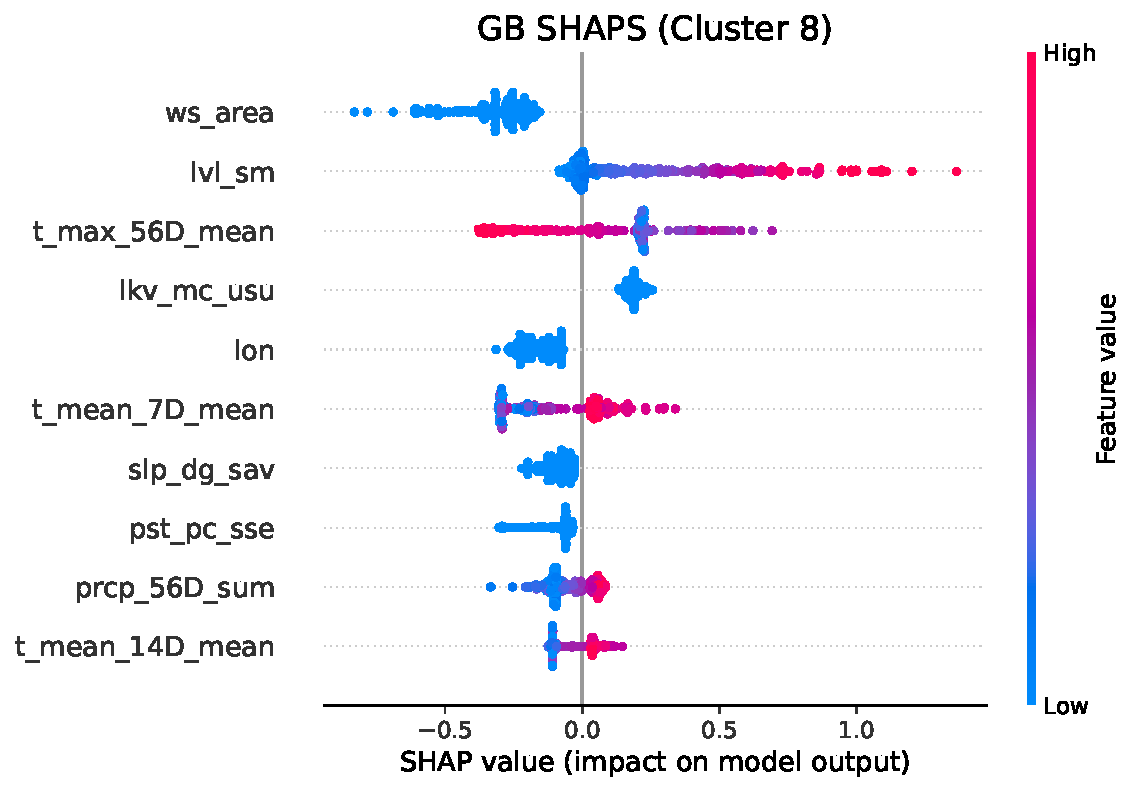
\includegraphics[width=\linewidth]{bin/shaps/gb/shap_top10_8.pdf} % Replace with your PDF file
        % \caption{Caption for Plot 9}
    \end{subfigure}

    \caption{SHAP values for Gradient boosting}
    \label{fig:shap_gb} % Label for cross-referencing the entire figure
\end{figure}

Figure~\ref{fig:shap_gb} shows the SHAP values for the Gradient Boosting model across all nine clusters. Unlike the Random Forest, we observe substantial variability in top features between clusters. While soil moisture level (lvl\_sm) still frequently appears in the top three, some clusters are dominated by maximum 56-day temperature (t\_max\_56D\_mean, e.g., clusters 0 and 7), others by watershed area (ws\_area, clusters 2 and 8) or slope gradient (slp\_dg\_sav, cluster 1). Precipitation dynamics (pst\_pc\_sse) rank highly only in a few clusters (1 and 8). This pattern suggests that Gradient Boosting better differentiates hydrological characteristics of individual basin groups, adapting to their specific local drivers.

\subsection{Metrics}

As shown in Figure~\ref{fig:results_metrics}, we evaluate model performance using four standard metrics --- Nash--Sutcliffe Efficiency (NSE), Root--Mean--Square Error (RMSE), Mean Absolute Error (MAE), and Mean Absolute Percentage Error (MAPE) --- for clusters 0--3.

\begin{enumerate}
    \item \textbf{Overall performance.} Across all clusters, the Random Forest consistently achieves higher NSE values and lower error magnitudes (RMSE, MAE, and MAPE) than the Gradient Boosting model. For example, in cluster 0 RF attains NSE = 0.922 versus GB's 0.780, while its RMSE (0.343 m\^3\/s) is roughly 40.
    \item \textbf{Cluster‐specific insights.} \begin{itemize}
              \item \emph{Cluster 1}: RF (NSE 0.909) greatly outperforms GB (0.634), with GB's MAPE exceeding 1 % due to occasional large percentage errors.
              \item \emph{Cluster 2}: Both models perform well (NSE > 0.8), but RF's mean errors (RMSE 0.112, MAE 0.052) remain smallest, reflecting accurate predictions even in basins with low discharge variability.
              \item \emph{Cluster 3}: The performance gap persists, with RF achieving NSE 0.939 and GB 0.829, and RF's MAE nearly half that of GB.
          \end{itemize}
    \item \textbf{Implications.} The superior and more stable skill of the Random Forest --- particularly its robustness against outliers (as evidenced by lower RMSE) --- suggests it as the preferred modeling approach for these hydrological clusters.
\end{enumerate}


\begin{figure}

    \begin{center}
        %----------- Gradient Boosting ---------------
        \textbf{Gradient Boosting}\\[0.2cm]
        \begin{tabular}{
                l    % cluster
                c    % NSE
                c    % RMSE
                c    % MAE
                c    % MAPE
                r    % n_samples
            }
            \toprule
            \textbf{cluster} & \textbf{NSE} & \textbf{RMSE} & \textbf{MAE} & \textbf{MAPE} & \textbf{Total basins} \\
            \midrule
            0                & 0.780        & 0.577         & 0.259        & 0.655         & 44\,544               \\
            1                & 0.634        & 0.372         & 0.143        & 1.228         & 38\,371               \\
            2                & 0.820        & 0.214         & 0.120        & 0.454         & 1\,096                \\
            3                & 0.829        & 0.708         & 0.325        & 1.093         & 12\,583               \\
            \bottomrule
        \end{tabular}

        \vspace{1.0em}  % small vertical gap

        %----------- Random Forest -------------------
        \textbf{Random Forest}\\[0.2cm]
        \begin{tabular}{
                l
                c
                c
                c
                c
                r
            }
            \toprule
            \textbf{cluster} & \textbf{NSE} & \textbf{RMSE} & \textbf{MAE} & \textbf{MAPE} & \textbf{Total basins} \\
            \midrule
            0                & 0.922        & 0.343         & 0.149        & 0.428         & 44\,544               \\
            1                & 0.909        & 0.185         & 0.070        & 0.590         & 38\,371               \\
            2                & 0.950        & 0.112         & 0.052        & 0.173         & 1\,096                \\
            3                & 0.939        & 0.424         & 0.158        & 0.653         & 12\,583               \\
            \bottomrule
        \end{tabular}
    \end{center}
    \label{fig:results_metrics}
    \caption{Result metrics}
\end{figure}

% % Experiment 3. LSTM
% % ————————————————————————————————————————————————————————————————————————————
% \subsection{Experiment 3. SARIMA}
% \label{experiment:SARIMA}


% % Experiment 4. LSTM
% % ————————————————————————————————————————————————————————————————————————————
% \subsection{Experiment 4. LSTM}
% \label{experiment:LSTM}
